\documentclass[conference]{IEEEtran}
\IEEEoverridecommandlockouts
% The preceding line is only needed to identify funding in the first footnote. If that is unneeded, please comment it out.
\usepackage{cite}
\usepackage{amsmath,amssymb,amsfonts}
\usepackage{algorithmic}
\usepackage{graphicx}
\usepackage{textcomp}
\usepackage{xcolor}
\usepackage{tikz}
\usepackage{subfig}
\usepackage{algorithm2e} % For algorithms
\def\BibTeX{{\rm B\kern-.05em{\sc i\kern-.025em b}\kern-.08em
    T\kern-.1667em\lower.7ex\hbox{E}\kern-.125emX}}
\begin{document}

\title{A Tethered Robot for COPD Patients}

\author{Luciano Bianchi, Esteban Alejandro Buniak~\IEEEmembership{Member,~IEEE,}, Rodrigo~Ramele,~\IEEEmembership{Member,~IEEE,}
        and Juan~Miguel~Santos% <-this % stops a space
\thanks{E. A. Buniak, R. Ramele  and J.M.Santos are with the CIC Laboratory at the Department
of  Computer Engineering, Instituto Tecnológico de Buenos Aires (ITBA), Ciudad de Buenos Aires,  Argentina e-mail: rramele@itba.edu.ar}% <-this % stops a space
\thanks{Manuscript received May 16, 2020; revised July 6, 2020.}}


\author{
\IEEEauthorblockN{1\textsuperscript{st} Luciano Bianchi}
\IEEEauthorblockA{\textit{CIC Laboratory at the Department
of  Computer Engineering} \\
\textit{Instituto Tecnológico de Buenos Aires (ITBA)}\\
Buenos Aires, Argentina \\
lbianchi@itba.edu.ar}
\and
\IEEEauthorblockN{2\textsuperscript{nd} Esteban Alejandro Buniak~\IEEEmembership{Member,~IEEE,}}
\IEEEauthorblockA{\textit{CIC Laboratory at the Department
of  Computer Engineering} \\
\textit{Instituto Tecnológico de Buenos Aires (ITBA)}\\
Buenos Aires, Argentina \\
ebuniak@itba.edu.ar}
\and
\IEEEauthorblockN{3\textsuperscript{rd} Rodrigo~Ramele,~\IEEEmembership{Member,~IEEE,}}
\IEEEauthorblockA{\textit{CIC Laboratory at the Department
of  Computer Engineering} \\
\textit{Instituto Tecnológico de Buenos Aires (ITBA)}\\
Buenos Aires, Argentina \\
rramele@itba.edu.ar}
\and
\IEEEauthorblockN{4\textsuperscript{th} Juan~Miguel~Santos}
\IEEEauthorblockA{\textit{CIC Laboratory at the Department
of  Computer Engineering} \\
\textit{Instituto Tecnológico de Buenos Aires (ITBA)}\\
Buenos Aires, Argentina \\
jsantos@itba.edu.ar}
}

\maketitle

\begin{abstract}
Patients that suffer Chronic Obstructive Pulmonary Disease (COPD) undergo a procedure called Pulmonary Rehabilitation that helps them to improve disease prognosis.  Pulmonary Rehabilitation consists of different physical exercises and walking activities conducted at medical facilities under supervision of a physical therapist.  In order to perform these procedures, patients require oxygen assistance, but the oxygen tank cannot be carried by the patient due to the musculoskeletal atrophy that characterize this pathology and external assistance is required.   The assistance to transport the bulky oxygen tank can be provided by a robotic device that follows the patient while performing the physical activities. This work provides an initial study on the controlling mechanism of a differential tethered robot that implements a leader-follower configuration to carry the oxygen tank for these procedures.  Results on a simulated and on a real prototype confirms the feasibility of the proposed solution.
\end{abstract}

% \begin{IEEEkeywords}
% component, formatting, style, styling, insert
% \end{IEEEkeywords}


\section{Introduction}
% The very first letter is a 2 line initial drop letter followed
% by the rest of the first word in caps.
% 
% form to use if the first word consists of a single letter:
% \IEEEPARstart{A}{demo} file is ....
% 
% form to use if you need the single drop letter followed by
% normal text (unknown if ever used by the IEEE):
% \IEEEPARstart{A}{}demo file is ....
% 
% Some journals put the first two words in caps:
% \IEEEPARstart{T}{his demo} file is ....
% 
% Here we have the typical use of a "T" for an initial drop letter
% and "HIS" in caps to complete the first word.

%The EEG is traditionally analyzed in terms of temporal waveforms at certain channels, looking at power of rhythms in the spontaneous EEG, at amplitude and latency of the peaks and troughs in event- related potentials (ERPs), or at particular grapho-elements in patho- logical or sleep stages.

\IEEEPARstart{C}{hronic} Obstructive Pulmonary Disease (COPD) is an umbrella term that describes several pulmonary affections.  They are characterized as a slowly progressive condition marked by airflow limitation, being cigarette smoking the main etiologic factor~\cite{MacNee2005}. This pathology presents a musculoskeletal atrophy~\cite{Kocsis2016,Wu2012}. In order to carve these after effects a Pulmonary Rehabilitation procedure is a viable treatment for patients.  Pulmonary Rehabilitation procedures consist of controlled walking activities and physical exercises that patients perform under the supervision of a physical therapist.  However, COPD patients present a severe low oxygen saturation illness and they require oxygen supply, particularly when performing physical activities~\cite{Celli2014}.  Hence, they are required to carry an oxygen tank for the oxygenotherapy assistance, but their own condition hinders their ability to precisely carry the often bulky external tank. 

This is a textbook situation when for an assitive ground service robot~\cite{Neto2015} to carry the oxygen tank while following the patient in a leader-follower configuration.  There are two reasons that support the initial viability of this idea.  First,  the rehabilitation gym is a constrained environment where this problem can be tackled by an Unmanned Ground Vehicle (UGV).  On the other hand, the range of movements performed by the patient during the Rehabilitation Procedure is highly predictable by the treatment. 

This work provides an initial study on the controlling mechanism of a differential tethered robot that implements the leader-follower configuration on a Pulmonary Rehabilitation procedure, following the line established by \cite{Endo2015}.  

\section{Materials and Methods}
\label{materials}

%This discipline is part of what is being called 4th industrial revolution and is reshaping many aspects of global manufacturing, including robotic and healthcare.

A basic robotic configuration is designed that allows quick prototyping and validation by the medical community.  This design is first simulated in a simulation environment, and later, a basic cost-wise hardware prototype based on Internet of Robotic Things~\cite{Simoens2018}  is built to verify the design guidelines and assumptions on a real world scenario.


\subsection{Solution Design}

The proposed solution is a Differential-Wheeled Robot (DWR) tethered to the followed subject with two threads ending at a single point attached to the subject waist, back or hand. In the same axis as the two front wheels, the robot has two reels separated by a certain length from which these threads come. As the subject moves away from the robot, the reels release thread so that the patient does not physically drag the vehicle. When the opposite happens, and the vehicle gets closer to the subject, an active spring mechanism driven by electric motors move each reel to retract the thread. The threads need to be tense at all times so that the encoders in each reel can be used to continuously measure the distance between the subject and the reel as devised in Figure~\ref{fig:components}.

% El detalle de los encoders se puede eliminar, es info común.
Encoders in each reel measure the difference in length of each thread compared to its initial position. These differences in length are the input for the control algorithm. The initial position of the threads is configurable.

% \subsection{Hardware}

\begin{figure}[h!]
\centering
\includegraphics[width=8cm]{images/alpibot1.jpg}
\caption{Side-view of the robot prototype.  A differential wheel, the reel and the rear free castor wheel can be observed from the picture.}
\label{fig:alpibot1}
\end{figure}



% \begin{figure*}[!t]
% \centering
% \subfloat{\includegraphics[width=15cm]{images/alpibot2.jpg}\label{subject8}}
% \caption{Top view of the robot prototype.  The SBC is shown on the center, alongside the Arduino Mega board.  Both reels can be seen on the same vertical plane of the wheel axis. A power bank (white) is located on one side of the robot, and on the rear part, the motor power battery (black) is located.}
% \label{fig:alpibot2}
% \end{figure*}


%The microcontroller is connected through serial connection to the main SBC RaspberryPi Model 3B+.  The main controlling algorithm run on this board, it connects to wifi and provides telemetry and the abiilty to receive remote commands by means a very simple UDP command interface.

% \subsection{Active Reel Spring}

% As previously mentioned, an active spring~\cite{Vanderborght2013} mechanism is also put in place to keep the threads tense.  However, in order to extend the useful life of the reel motors, and to save battery, an algorithm to  activate and deactivate the motors was developed. 

% The algorithm works as follows: 

% \begin{enumerate}
%     \item While wheels are moving, retract reels.
%     \item If wheels stop moving, wait for \textit{reel wait time} seconds, then retract reels. 
%     \item Retract reels until the reel encoders values have not changed during \textit{reel retract time} seconds.
%     \item If wheels started moving or the encoder values have changed while retracting, start the \textit{reel retract time} countdown again.
% \end{enumerate}{}

%Here is the pseudocode that implements that logic. This function is executed in every run loop in the Arduino module:


%\begin{algorithm}[]
%\label{alg:active_spring}
%\caption{Active spring algorithm}
%\begin{algorithmic}
%
%\STATE $currentReelPulses \gets readPulses()$
%
%\IF{$retracting$}
%    \IF{$lastReelPulses != currentReelPulses$}
%    \STATE $lastReelStart \gets currentTime()$
%    \ENDIF
%    \IF{\NOT $ wheelsMoving $ \AND $ currentTime() - lastReelStart > rrt$}
%    \STATE $retracting \gets \FALSE$
%    \STATE $lastReelEnd \gets currentTime()$
%    \ENDIF
%\ELSE
%    \IF{$wheelsMoving$}
%        \STATE $retracting \gets \TRUE$
%        \STATE $lastReelStart \gets currentTime()$
%    \ENDIF
%    \IF{$ currentTime() - lastReelEnd > rwt $}
%        \STATE $retracting \gets \TRUE$
%        \STATE $lastReelStart \gets currentTime()$
%    \ENDIF
%\ENDIF
%
%\STATE $lastReelPulses \gets currentReelPulses$
%
%\IF{$retracting$}
%    \STATE \textit{Activate reel motors}
%\ELSE
%    \STATE \textit{Deactivate reel motors}
%\ENDIF
%\end{algorithmic}
%\end{algorithm}


%\subsection{Software Components}

\subsection{Control Strategy}

The main control strategy proposed in this work, that we called \textit{Follow the Thread}, is similar to the one presented in \cite{Ortlieb2016}.  It is based on the idea that both the relative angle between the subject and the vehicle orientation and, the relative distance between the robot and the subject, can be computed from the length of the left and right threads.  They are described by Equations~\ref{eq:lemniscata}, \ref{eq:lemniscata2} and~\ref{eq:lemniscata3}.

\begin{equation}
V_t = c_v (\frac{l_L + l_R}{2} - l_D)
\label{eq:lemniscata}
\end{equation}

\begin{equation}
\omega_{L} = V_t + c_{\alpha} (l_L - l_R)
\label{eq:lemniscata2}
\end{equation}

\begin{equation}
\omega_{R} = V_t - c_{\alpha} (l_L - l_R)
\label{eq:lemniscata3}
\end{equation}

\noindent where  $c_v$ and $c_{\alpha}$ are constant coefficients used for calibration whose units are expressed in $[\frac{1}{s}]$, and $l_D$ is a constant offset in $[m]$ that is used to customize the desired length of the thread where the robot does not move.   As shown on Figure~\ref{fig:follow_params},  $l_L$ and $l_R$ are changes in the length of thread that was released from each reel in $[m]$  obtained from encoder information, $V_t$ is the estimated forward velocity for the target and finally $\omega_{L}$ are $\omega_{R}$ are the velocity values that are directly used to drive each wheel motor.

To stop the vehicle completely when it is close to its expected position, an additional condition is added: 

\begin{equation}
\textit{if  }{\frac{l_L + l_R}{2} < l_D}\textit{ then } \omega_{L} = \omega_{R} = 0.
\end{equation}

\begin{figure}[]
    \centering
    \tikzset{every picture/.style={line width=0.75pt}} %set default line width to 0.75pt        
    
    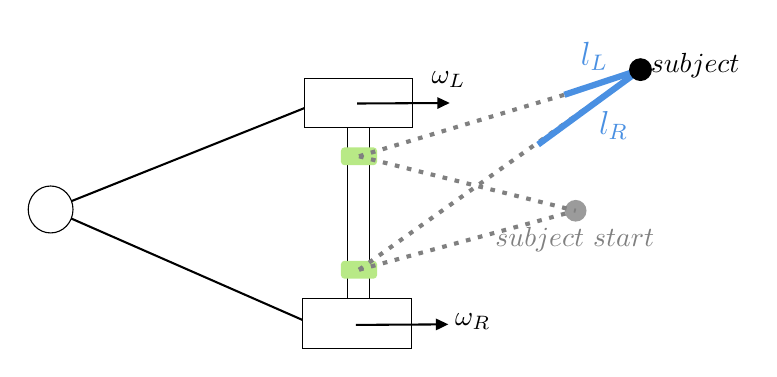
\begin{tikzpicture}[x=0.50pt,y=0.50pt,yscale=-1,xscale=1]
    %uncomment if require: \path (0,2317); %set diagram left start at 0, and has height of 2317
    
    %Shape: Rectangle [id:dp785217180323701] 
    \draw   (332,1925.29) -- (347.46,1925.29) -- (347.46,2120.1) -- (332,2120.1) -- cycle ;
    %Straight Lines [id:da8987873257842873] 
    \draw [color={rgb, 255:red, 0; green, 0; blue, 0 }  ,draw opacity=1 ][line width=0.75]    (300.46,2100.29) -- (117.19,2019.9) ;
    %Straight Lines [id:da585150688871364] 
    \draw [color={rgb, 255:red, 0; green, 0; blue, 0 }  ,draw opacity=1 ][fill={rgb, 255:red, 230; green, 164; blue, 164 }  ,fill opacity=1 ][line width=0.75]    (301.46,1946.29) -- (117.19,2019.9) ;
    %Shape: Rectangle [id:dp8556526042433679] 
    \draw  [fill={rgb, 255:red, 255; green, 255; blue, 255 }  ,fill opacity=1 ] (300.5,1925) -- (379,1925) -- (379,1960.67) -- (300.5,1960.67) -- cycle ;
    %Shape: Ellipse [id:dp024503202773356936] 
    \draw  [color={rgb, 255:red, 0; green, 0; blue, 0 }  ,draw opacity=1 ][fill={rgb, 255:red, 255; green, 255; blue, 255 }  ,fill opacity=1 ] (101.01,2019.9) .. controls (101.01,2010.53) and (108.25,2002.94) .. (117.19,2002.94) .. controls (126.12,2002.94) and (133.37,2010.53) .. (133.37,2019.9) .. controls (133.37,2029.28) and (126.12,2036.87) .. (117.19,2036.87) .. controls (108.25,2036.87) and (101.01,2029.28) .. (101.01,2019.9) -- cycle ;
    %Shape: Rectangle [id:dp4521863424396907] 
    \draw  [fill={rgb, 255:red, 255; green, 255; blue, 255 }  ,fill opacity=1 ] (299.5,2084.5) -- (378,2084.5) -- (378,2120.17) -- (299.5,2120.17) -- cycle ;
    %Rounded Rect [id:dp9798921511906625] 
    \draw  [draw opacity=0][fill={rgb, 255:red, 184; green, 233; blue, 134 }  ,fill opacity=1 ] (327,2059.58) .. controls (327,2058.16) and (328.16,2057) .. (329.58,2057) -- (350.53,2057) .. controls (351.96,2057) and (353.11,2058.16) .. (353.11,2059.58) -- (353.11,2067.34) .. controls (353.11,2068.76) and (351.96,2069.92) .. (350.53,2069.92) -- (329.58,2069.92) .. controls (328.16,2069.92) and (327,2068.76) .. (327,2067.34) -- cycle ;
    %Rounded Rect [id:dp969028519585216] 
    \draw  [draw opacity=0][fill={rgb, 255:red, 184; green, 233; blue, 134 }  ,fill opacity=1 ] (327,1977.58) .. controls (327,1976.16) and (328.16,1975) .. (329.58,1975) -- (350.53,1975) .. controls (351.96,1975) and (353.11,1976.16) .. (353.11,1977.58) -- (353.11,1985.34) .. controls (353.11,1986.76) and (351.96,1987.92) .. (350.53,1987.92) -- (329.58,1987.92) .. controls (328.16,1987.92) and (327,1986.76) .. (327,1985.34) -- cycle ;
    %Straight Lines [id:da8580549640030513] 
    \draw [color={rgb, 255:red, 128; green, 128; blue, 128 }  ,draw opacity=1 ][line width=1.5]  [dash pattern={on 1.69pt off 2.76pt}]  (340.06,2063.46) -- (496.67,2020.83) ;
    %Shape: Circle [id:dp1613016595870852] 
    \draw  [draw opacity=0][fill={rgb, 255:red, 155; green, 155; blue, 155 }  ,fill opacity=1 ] (488.83,2020.83) .. controls (488.83,2016.51) and (492.34,2013) .. (496.67,2013) .. controls (500.99,2013) and (504.5,2016.51) .. (504.5,2020.83) .. controls (504.5,2025.16) and (500.99,2028.67) .. (496.67,2028.67) .. controls (492.34,2028.67) and (488.83,2025.16) .. (488.83,2020.83) -- cycle ;
    %Straight Lines [id:da10232028406547378] 
    \draw [color={rgb, 255:red, 0; green, 0; blue, 0 }  ,draw opacity=1 ][line width=0.75]    (338.75,1943.33) -- (402.58,1942.95) ;
    \draw [shift={(405.58,1942.93)}, rotate = 539.65] [fill={rgb, 255:red, 0; green, 0; blue, 0 }  ,fill opacity=1 ][line width=0.08]  [draw opacity=0] (8.93,-4.29) -- (0,0) -- (8.93,4.29) -- cycle    ;
    %Straight Lines [id:da5543519847675118] 
    \draw [color={rgb, 255:red, 0; green, 0; blue, 0 }  ,draw opacity=1 ][line width=0.75]    (337.75,2103.33) -- (401.58,2102.95) ;
    \draw [shift={(404.58,2102.93)}, rotate = 539.65] [fill={rgb, 255:red, 0; green, 0; blue, 0 }  ,fill opacity=1 ][line width=0.08]  [draw opacity=0] (8.93,-4.29) -- (0,0) -- (8.93,4.29) -- cycle    ;
    %Straight Lines [id:da5830729933065488] 
    \draw [color={rgb, 255:red, 128; green, 128; blue, 128 }  ,draw opacity=1 ][line width=1.5]  [dash pattern={on 1.69pt off 2.76pt}]  (340.06,1981.46) -- (496.67,2020.83) ;
    %Straight Lines [id:da27552399356884627] 
    \draw [color={rgb, 255:red, 128; green, 128; blue, 128 }  ,draw opacity=1 ][line width=1.5]  [dash pattern={on 1.69pt off 2.76pt}]  (340.06,1981.46) -- (488.5,1937) ;
    %Straight Lines [id:da06167712807711301] 
    \draw [color={rgb, 255:red, 128; green, 128; blue, 128 }  ,draw opacity=1 ][line width=1.5]  [dash pattern={on 1.69pt off 2.76pt}]  (340.06,2063.46) -- (543.5,1918.83) ;
    %Straight Lines [id:da887785453759708] 
    \draw [color={rgb, 255:red, 74; green, 144; blue, 226 }  ,draw opacity=1 ][line width=2.25]    (488.5,1937) -- (543.5,1918.83) ;
    %Straight Lines [id:da7211287180458504] 
    \draw [color={rgb, 255:red, 74; green, 144; blue, 226 }  ,draw opacity=1 ][line width=2.25]    (469.5,1973) -- (543.5,1918.83) ;
    %Shape: Circle [id:dp7802267148020259] 
    \draw  [fill={rgb, 255:red, 0; green, 0; blue, 0 }  ,fill opacity=1 ] (535.67,1918.83) .. controls (535.67,1914.51) and (539.17,1911) .. (543.5,1911) .. controls (547.83,1911) and (551.33,1914.51) .. (551.33,1918.83) .. controls (551.33,1923.16) and (547.83,1926.67) .. (543.5,1926.67) .. controls (539.17,1926.67) and (535.67,1923.16) .. (535.67,1918.83) -- cycle ;
    
    % Text Node
    \draw (524,1960) node  [font=\large,color={rgb, 255:red, 74; green, 144; blue, 226 }  ,opacity=1 ]  {$ \begin{array}{l}
    l_{R}\\
    \end{array}$};
    % Text Node
    \draw (510,1910) node  [font=\large,color={rgb, 255:red, 74; green, 144; blue, 226 }  ,opacity=1 ,rotate=-358.27]  {$ \begin{array}{l}
    l_{L}\\
    \end{array}$};
    % Text Node
    \draw (496,2042) node  [color={rgb, 255:red, 128; green, 128; blue, 128 }  ,opacity=1 ]  {$subject\ start$};
    % Text Node
    \draw  [draw opacity=0][fill={rgb, 255:red, 255; green, 255; blue, 255 }  ,fill opacity=1 ]  (554.5,1904) -- (611.5,1904) -- (611.5,1928) -- (554.5,1928) -- cycle  ;
    \draw (583,1916) node    {$subject$};
    % Text Node
    \draw (390.58,1925.93) node [anchor=west] [inner sep=0.75pt]  [font=\normalsize,color={rgb, 255:red, 0; green, 0; blue, 0 }  ,opacity=1 ]  {$\omega_{L}$};
    % Text Node
    \draw (407.58,2100.93) node [anchor=west] [inner sep=0.75pt]  [font=\normalsize,color={rgb, 255:red, 0; green, 0; blue, 0 }  ,opacity=1 ]  {$\omega_{R}$};
    
    
    \end{tikzpicture}
    \caption{Following mechanism parameters}
    \label{fig:follow_params}
\end{figure}{}

% \subsection{Design comparison}

% In the scheme proposed by~\cite{Endo2015} a single thread is recovered mechanically by means of a circular flat spring. This device works intensively when the robot is following the patient and, therefore, the spring is exposed to wear. Additionally with a circular flat spring the properties of the spring components are predefined by their structural preconditions, and cannot be altered during spring operation~\cite{wurmthaler2013apparatus}. For instance, the spring tension depends on the released thread length, hence the recovery force will vary accordingly.  If the patient found this tension to be too tight, it is not possible to alter this behavior without structurally modifying the device, or changing the spring component altogether.  Instead, the double thread tethered design implemented with an active reel spring allows a more controlled situation and depends exclusively on the software that controls the reel motor, which can be regulated. 

% Regarding the control algorithm, authors in \cite{Endo2015} introduced two methods. The first of them computes the angular velocity as a function of the difference between the measured thread length $l_m$ and the desired distance to patient  $l_D$. In this way, if the patient moves around the robot with a $l_m$ equals to $l_D$, the robot will not adjust its direction until the patient stops turning and restarts moving forward. Hence, the robot must correct its direction but the correction angle could be large, which leads the robot to deviate off the desired trajectory. Additionally, the second method proposed is based on dead-reckoning to estimate the patient position. It is well stated~\cite{DurrantWhyte1994} that position estimation using dead-reckoning leads to an increasing error along cumulative distance with continuous changes of angular velocity. This presents a limitation to hold therapy sessions with patients who need to cover standard trajectory distances, requiring more frequent interruptions to perform calibration procedures.

%Another issue that can be presented is when $l_m$ is equals to $l_D$.  If the patient performs a circular movement where these values are equal, the robot will not change direction at all, because $\omega_{r}$ will be also zero.   If the patient restart the movement, $\omega_{r}$ could be very low and the proportional gain $K_p$ could not be enough to match the person movement rapidly.

%Additionally, authors in~\cite{Endo2015} propose an alternative control strategy based on dead-reckoning requires very precise measurements to reduce the error-prone characteristic of this solution~\cite{DurrantWhyte1994}.

%Otro problema que encontré es en el segundo método de control. Éste es un poco más complicado de explicar con palabras así que haré un gráfico y se los envío. Como adelanto, está en la ecuación 17 del paper que es cuando toman como medida de la diferencia de distancias (l_m - l_D) para el cálculo de la V_r.


%Por último, un problema del algoritmo de control de los tipos (el de follow-the-leader) es que está basado en "dead-reckoning" el cual es un método impreciso cuyo error crece a lo largo del tiempo. Esto es, la estrategia de los tipos es ir estimando la posición del paciente en base a la posición del robot en un sistema de coordenadas universal (no en el sistema de coordenadas cuyo centro es el robot). Esta estimación la obtienen, entiendo yo, basado en la información de los encoders de los motores del robot (ahí es donde meten la pata) y sumándole un vector que obtienen al rotar (l_m, 0) mediante una matriz de rotación con el ángulo expresado en el sistema de referencia universal). Es importante remarcar que su estrategia se basa en esto: en poder estimar la posición del paciente e ir guardándola (para luego estimar T(s_t const) y para eso usan dead reckoning, es decir, a medida que pasa el tiempo (en rigor, a medida que mayor longitud recorren) peor será la estimación y peor andará el algoritmo. Es cierto que en las curvas no se vé eso, pero también es cierto que, en una sesión terapéutica, recorran más distancia que las mostradas en los test.


\section{Experimental Protocol} \label{experimental}

This section describes the experimental protocol used to evaluate the performance of the proposed solution.  The Pulmonary Rehabilitation procedure consists on a series of walking activities aimed to promote patient muscular recovery and well being~\cite{Wu2012}. They are slow pace motions following a specific trajectory on a rehabilitation gym.

In order to standardize the procedure~\cite{Sprunk2016}, we define the desired trajectory as a curve shaped like an $\infty$ symbol, described by the Equations~\ref{eq:lemniscate}:

\begin{equation}
\begin{array}{ll}  
 x( \phi ) = a \; cos( \phi )     \\
 y( \phi ) = a \; cos ( \phi )   \; sin ( \phi )    \\ 
 \textit{where}  \; \phi \in \lbrace -\pi , \pi  \rbrace
\end{array}
\label{eq:lemniscate}
\end{equation}

\noindent where $ \phi $ is the free parameter, $a$ is the limit length of the arc of the curve, and $x$ and $y$ are the parametric functions that determine the shape of the trajectory on the navigation plane.

The reason  this shape was chosen is because it combines different kinds of trajectories where the vehicle can be tested: long straight segments, sharp and soft curves, all in one single shape. Similar curves are also used in other proposed experiments in \cite{Neto2015,Endo2015}.  

Regarding metrics, four are proposed to evaluate the performance.  They are:

DEJA UNA SOLA !!!!!

\begin{itemize}
    \item \textit{Normal trajectory deviation, n.t.d.}: the subject trajectory is divided into small segments and then the normal distance to the robot trajectory is calculated for each of those segments. Trajectory deviation curve is relevant to evaluate how closely the robot mimics the leader trajectory, which is the ultimate goal of the robotic vehicle. 
    \item \textit{Robot-leader distance, r.l.d.}: The euclidean distance between the robot and the leader, at any point in time. This curve is particularly important since the robot has a limited amount of thread available, so if the leader uses all the available thread, it will start dragging the robot and damaging the following mechanism, and overall it may rise the possibility of disconnecting the breathing oxygen cannula. This is a scenario that must not happen under any circumstance, as it can also be dangerous for a potential patient using the device. 
    \item \textit{Total trajectory deviation, t.t.d.}: The area under the curve resulting from the the \textit{normal trajectory deviation} over the length traveled by the leader.
    \item \textit{Maximum trajectory deviation, m.t.d.}: the maximum \textit{normal trajectory deviation} registered during an experiment.    
\end{itemize}{}

% In this work, a \textit{following behavior} is considered satisfactory if its maximum trajectory deviation is less than 0.75 m and the robot-leader distance never exceeds 1.5 m~\cite{MunozCeballos2010}.

% First the simulation is described and later the evaluation on the robotic prototype is detailed.

\subsection{Simulation}

A model of the proposed design was first built on Webots~\cite{Michel2004} simulator.  The threading mechanism was implemented using virtual threads~\cite{Rekleitis2001}.  The leader traveled according to a predefined trajectory with constant velocity, following the curve trajectory.

\subsection{Real world}


%To verify the validity of the proposed framework and method,
%The experimental protocol used to 
%In order to assess 

A real world experiment was performed, pegging to the same conditions implemented on the simulation environment.  A motion capture system is used to track the movement of a human leader along a predetermined trajectory.   

As shown on Figure~\ref{fig:capturesystem}, a tracking marker was placed on each side of the robot (on top of each thread reel). The human leader used his hand to grab the tip at which the two tethers were tied together. A third marker was placed in his hand, using a glove. A predetermined path was marked on the floor, and the human leader tried to move his hand following this shape as close as possible, with stable speed. 

\begin{figure}[h!]
\centering
\includegraphics[width=8cm]{images/capture.png}
\caption{Hardware prototype on the motion capture system and a testing subject holding the threads.}
\label{fig:capturesystem}
\end{figure}



\section{Results} \label{Results}
\label{results}

% Simulation results for both control strategies are shown on Figure~\ref{fig:simulationresults}. Subfigures (a) and (b) expound the trajectories of the leader and the follower for each strategy, while (c) and (d) describe their speed profiles.  Subfigure (e) show the distance between the robot and the patient for both strategies.  Results metrics for the simulations are shown on Table~\ref{tab:simulationmetricsftt} for the \textit{Follow the thread} strategy, whereas metrics for \textit{Rotate and go} are shown on Table~\ref{tab:simulationmetricsrg}.


\begin{center}
\begin{tabular}{ |c|c|c|c| }
\hline
$c_v$ & $c_{\alpha}$ & m.t.d. & t.t.d. \\
\hline
10  &   15  & 0.3614 & 2.0651\\
15  &   5  & 0.4325 & 2.055\\
\textbf{15}  &   \textbf{10}  & \textbf{0.2188} & \textbf{1.0902}\\
15  &   15  & 0.2891 & 1.5059\\
5  &   20  & 0.5733 & 3.7289\\
\hline
\end{tabular}
\captionof{table}{Maximum trajectory deviation m.t.d. (m) and Total trajectory deviation t.t.d. for different \textit{Follow the thread} constants.}
\label{tab:simulationmetricsftt}
\end{center}


%\begin{figure}[h!]
%\centering
%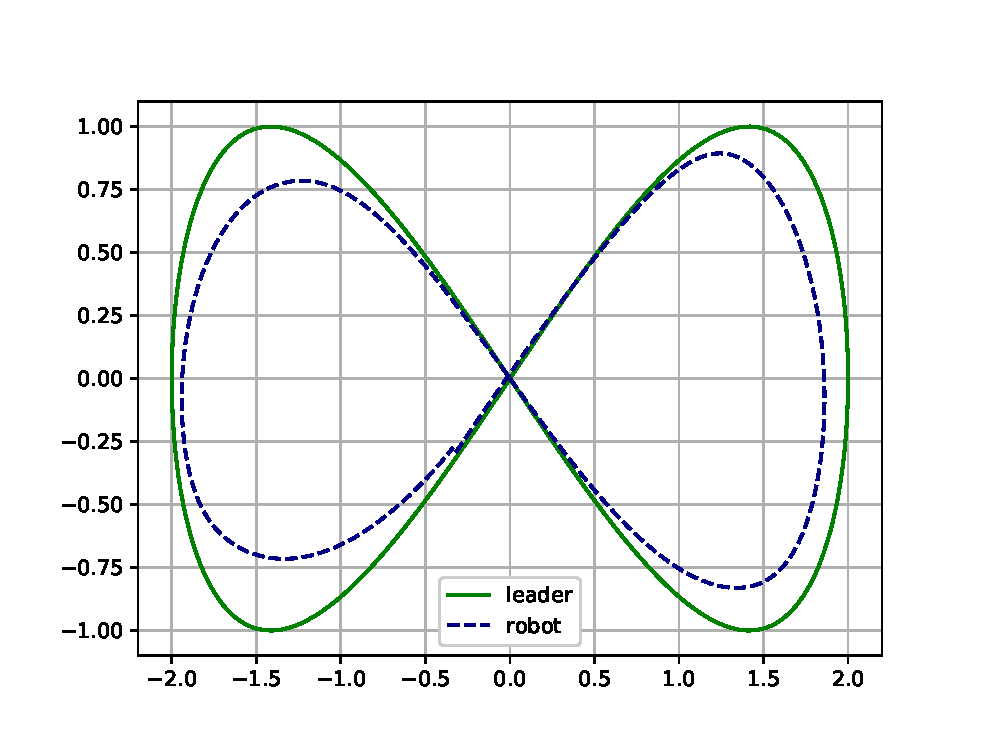
\includegraphics[width=8cm]{images/ft_a2_n1500_cv15_cr15.eps}
%\caption{Trajectories of the leader and follower for the \textit{Follow the thread} control strategy.}
%\label{fig:distance_sim}
%\end{figure}
%
%\begin{figure}[h!]
%\centering
%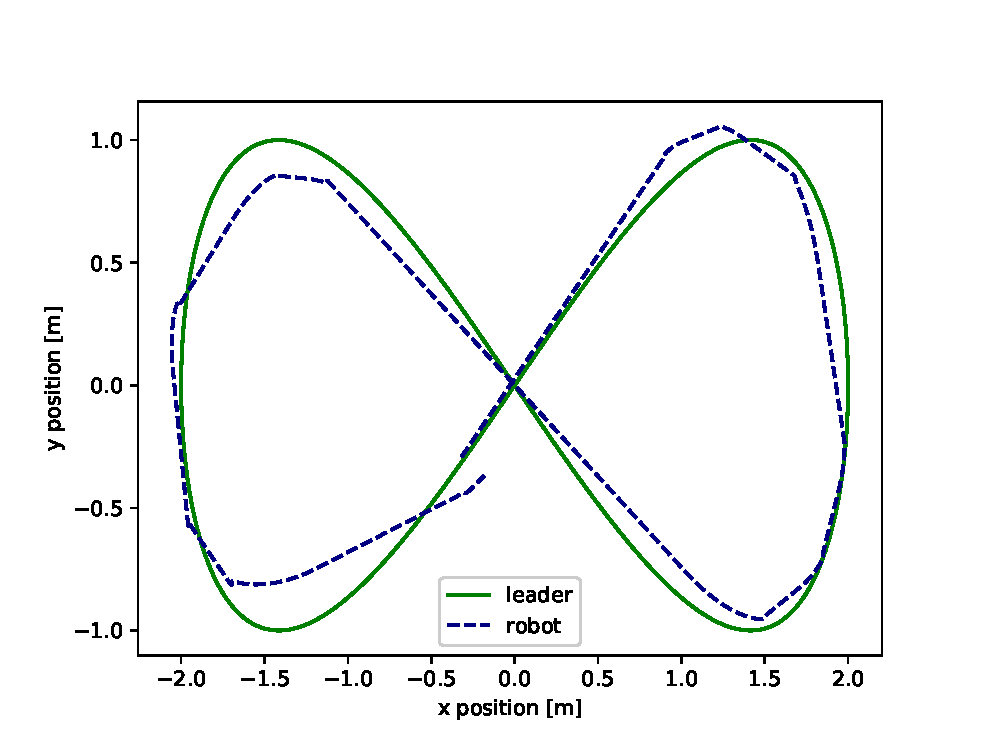
\includegraphics[width=8cm]{images/rgv_cv20_cr20_dr10.eps}
%\caption{Trajectories of the leader and follower for \textit{Rotate and go} control strategy.}
%\label{fig:distance_sim}
%\end{figure}
%
%\begin{figure}[h!]
%\centering
%\includegraphics[width=8cm]{images/ft_cv15_cr10_leader_robot_speed.eps}
%\caption{Speed profiles of the leader and follower for \textit{Follow the thread} control strategy.}
%\label{fig:distance_sim}
%\end{figure}
%
%\begin{figure}[h!]
%\centering
%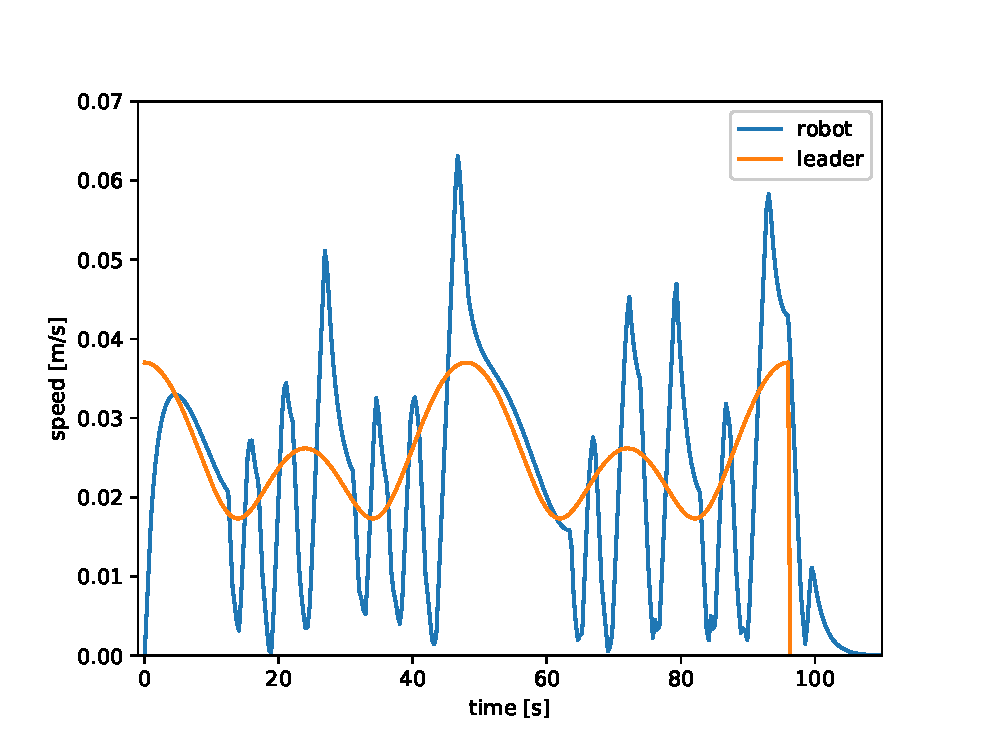
\includegraphics[width=8cm]{images/rg_cv20_cr20_bv10_dtoff10_leader_robot_speed.eps}
%\caption{Speed profiles of the leader and follower for \textit{Rotate and go} control strategy.}
%\label{fig:distance_sim}
%\end{figure}
%
%\begin{figure}[h!]
%\centering
%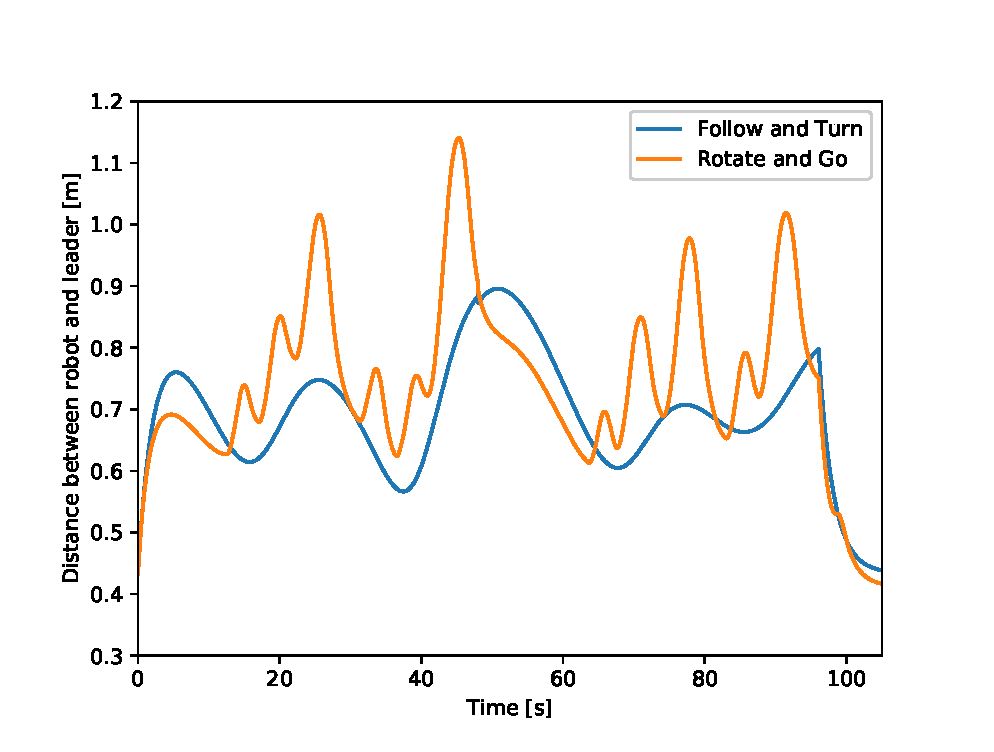
\includegraphics[width=8cm]{images/ft_vs_rg_dist.eps}
%\caption{Separation distance between robot and leader for both strategies [m].}
%\label{fig:distance_sim}
%\end{figure}


\begin{figure} 
    \centering
  \subfloat[ \label{sr1a}]{%
       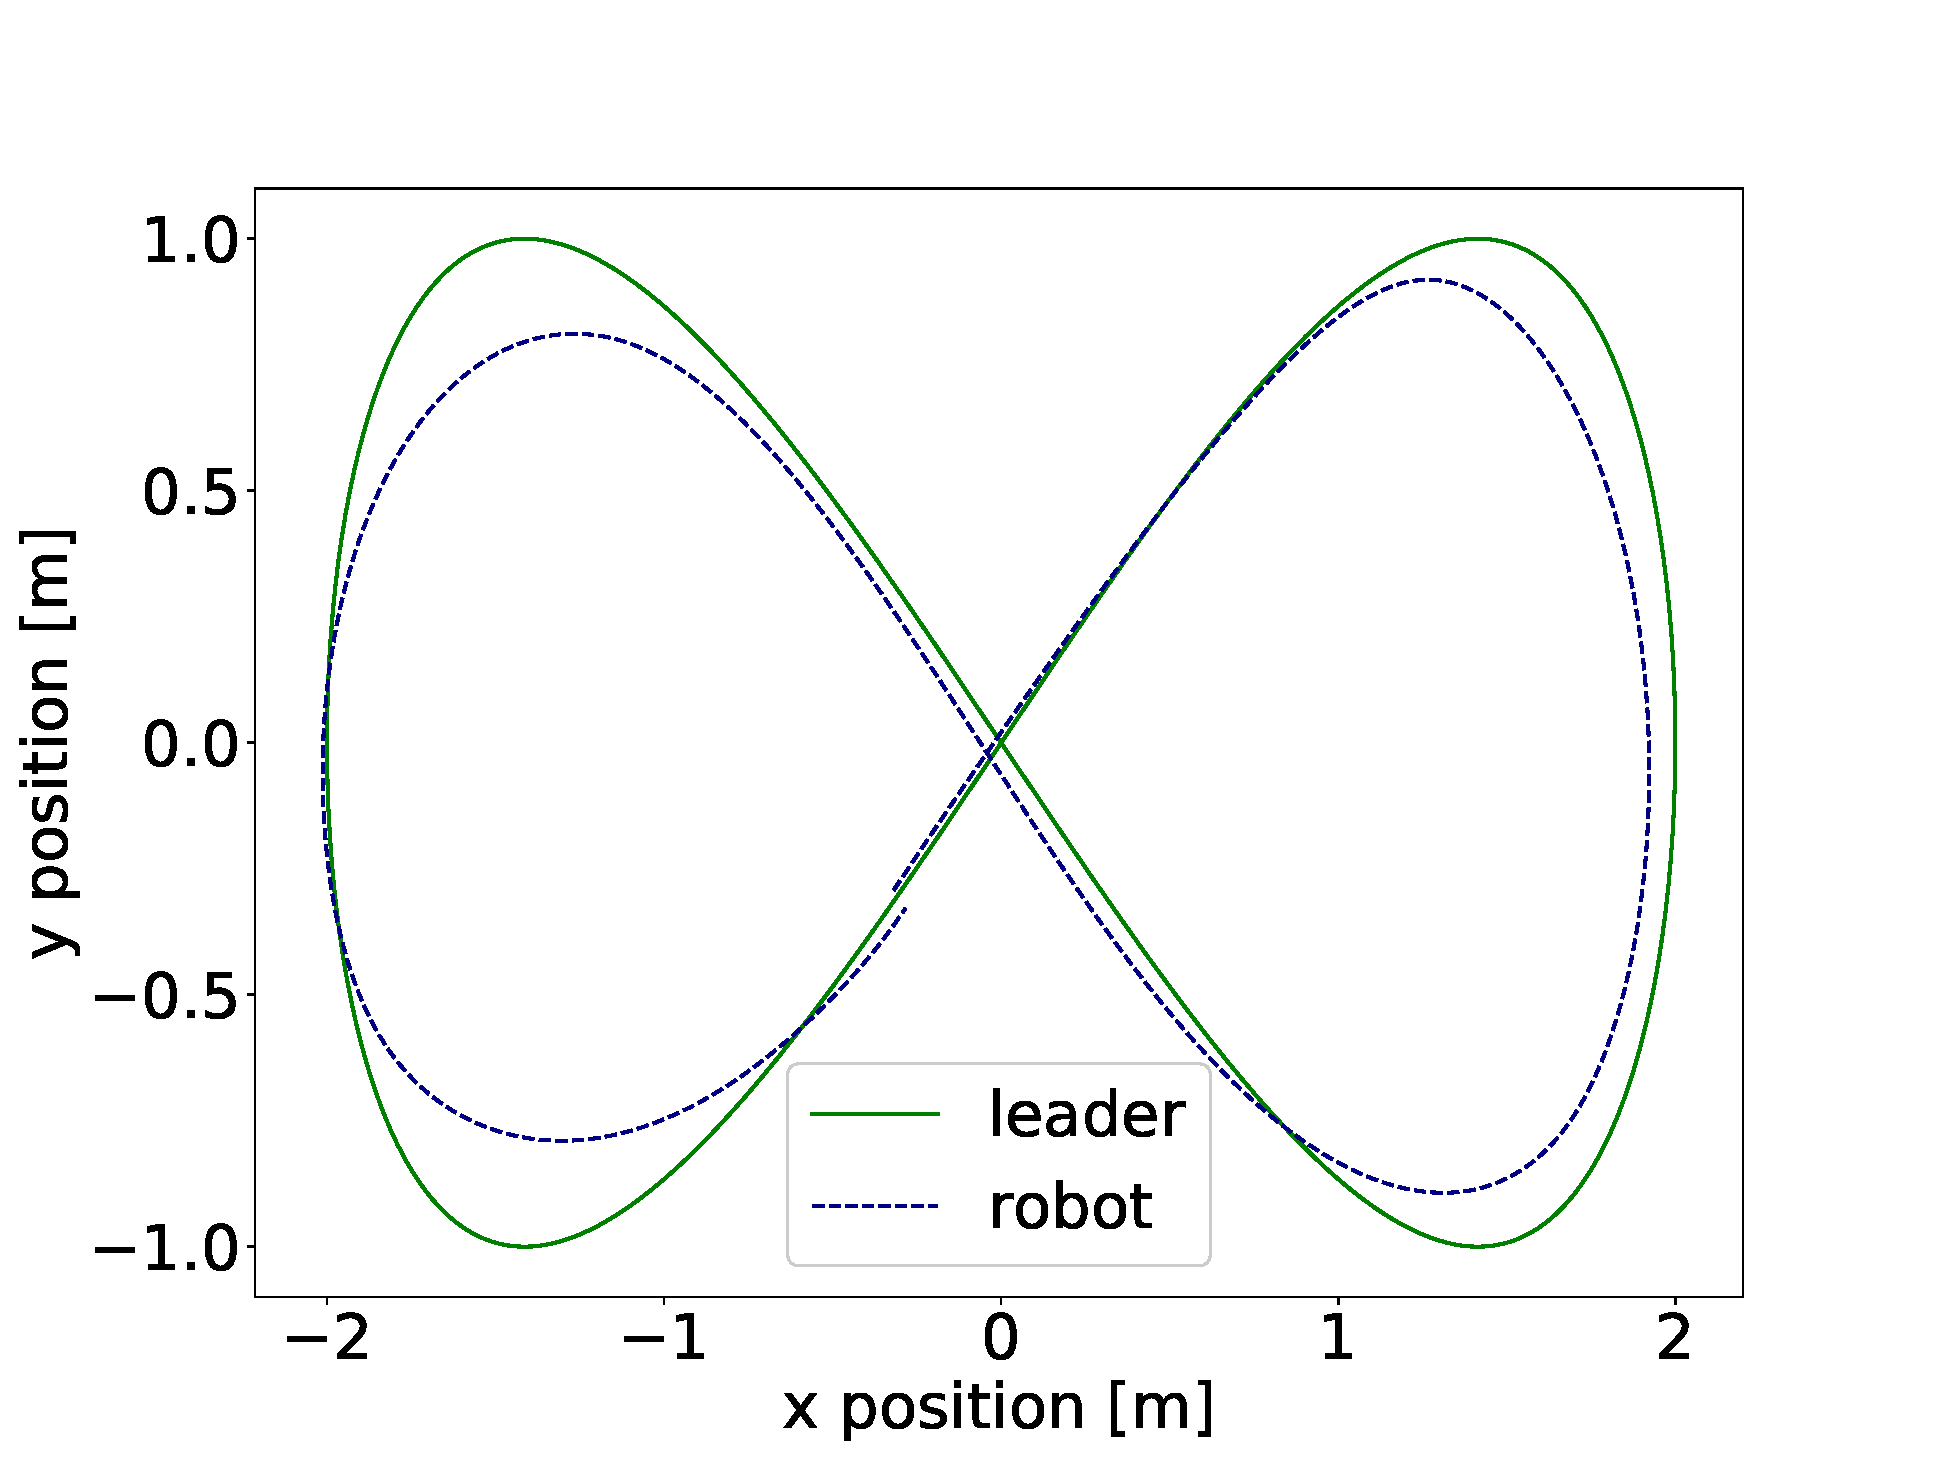
\includegraphics[width=0.8\linewidth]{images/simulation_follow-thread.eps}}
    \hspace*{-1.5em}
  \label{fig:simulationresults} 
\end{figure}



% Results for the real world experiment can be seen on Figure~\ref{fig:realworldresults}.   Table~\ref{tab:cap_ft_npd_table} shows the metrics of the \textit{Follow the thread} strategy, whereas Table~\ref{tab:cap_rg_npd_table} provides the metrics for the \textit{Rotate and go} approach.

%\begin{figure}[h!]
%\centering
%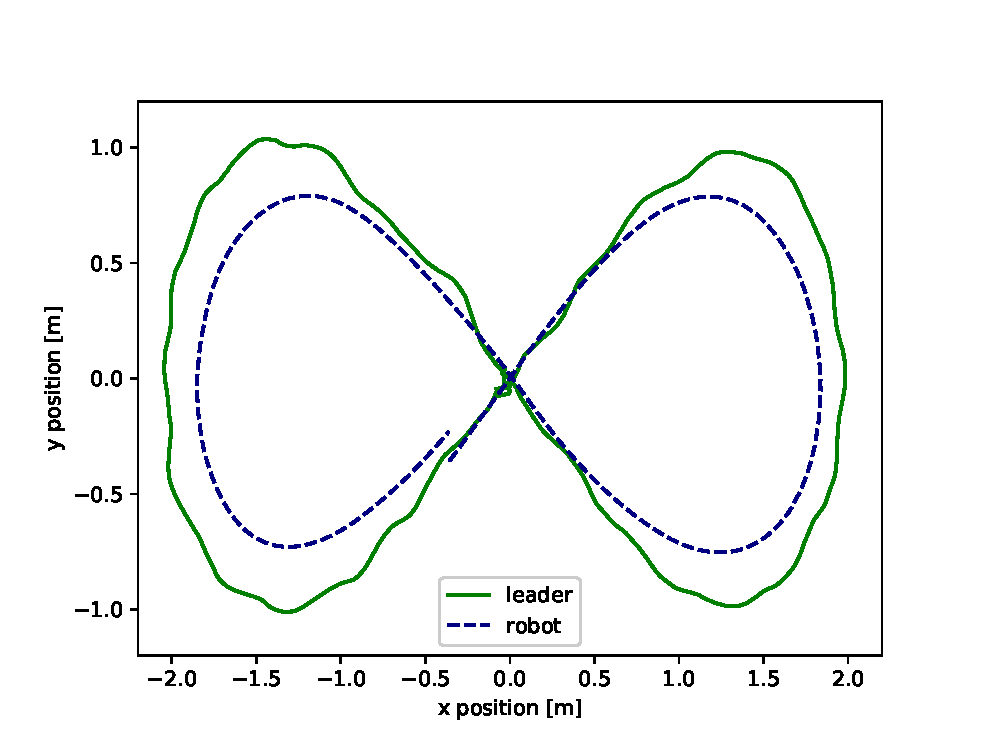
\includegraphics[width=8cm]{images/ft1cap.eps}
%\caption{Trajectories for the \textit{Follow the thread} control strategy.}
%\label{fig:distance_sim}
%\end{figure}
%
%
%\begin{figure}[h!]
%\centering
%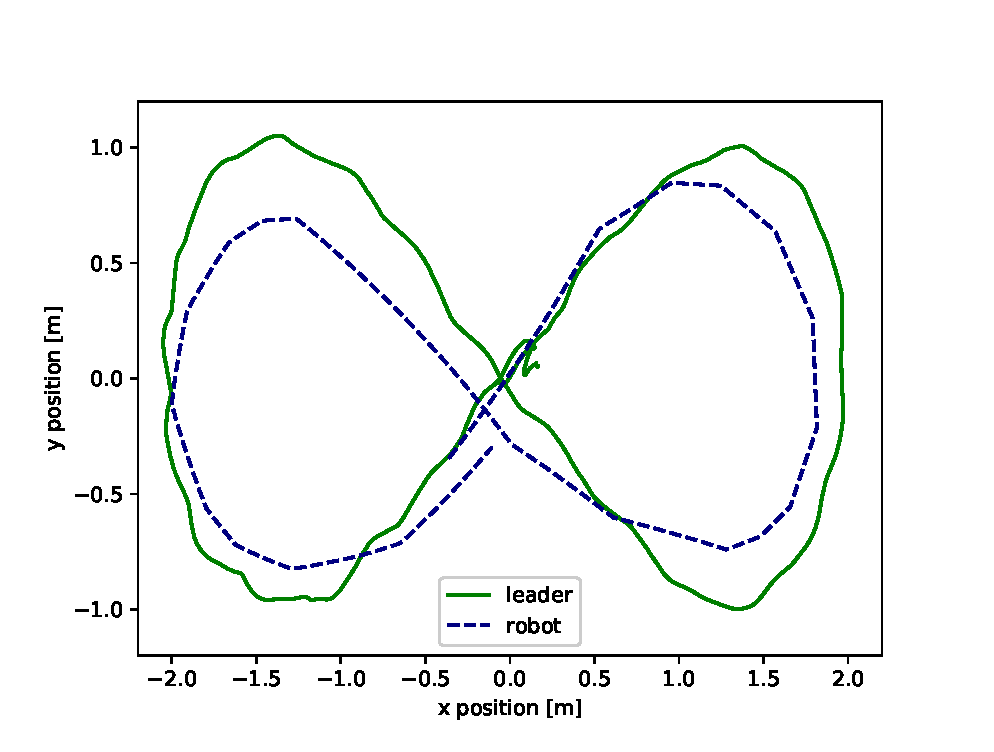
\includegraphics[width=8cm]{images/rg2cap.eps}
%\caption{Distance between robot and leader [m]}
%\label{fig:distance_sim}
%\end{figure}
%
%
%\begin{figure}[h!]
%\centering
%\includegraphics[width=8cm]{images/ft1cap_leader_robot_speed.eps}
%\caption{\textit{Follow the thread} speed profiles}
%\label{fig:distance_sim}
%\end{figure}
%
%
%\begin{figure}[h!]
%\centering
%\includegraphics[width=8cm]{images/rg2cap_leader_robot_speed.eps}
%\caption{Rotate and go speed profiles}
%\label{fig:distance_sim}
%\end{figure}
%
%
%\begin{figure}[h!]
%\centering
%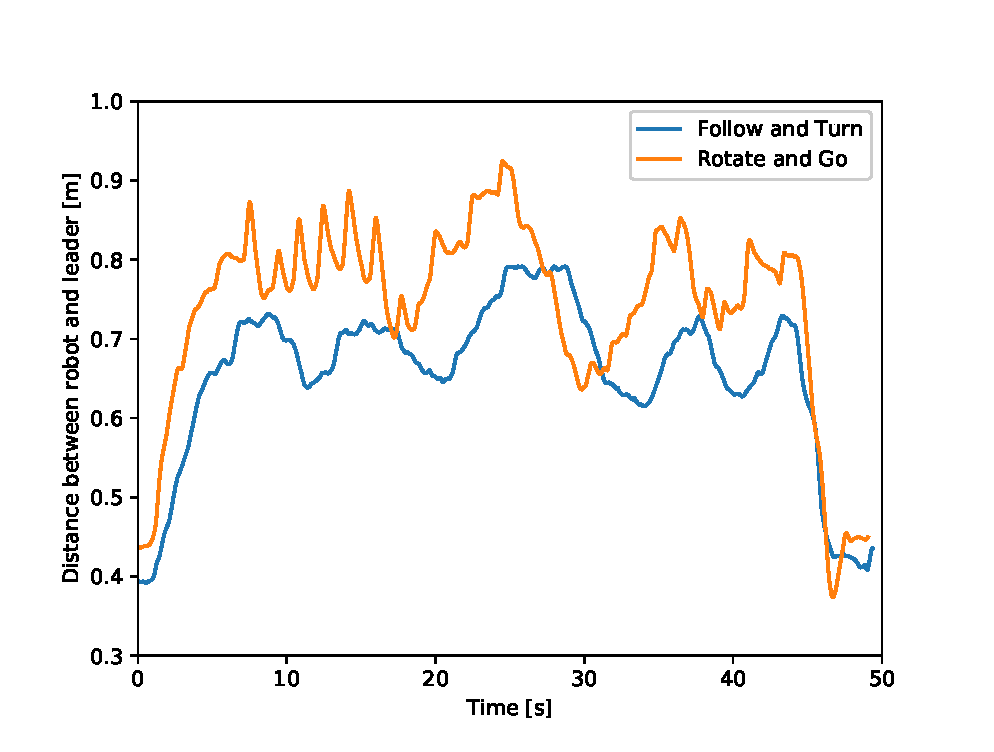
\includegraphics[width=8cm]{images/cap_ft_vs_rg_dist.eps}
%\caption{\textit{Rotate and go} speed profiles}
%\label{fig:distance_sim}
%\end{figure}


\begin{figure} 
    \centering
  \subfloat[ \label{rw1a}]{%
       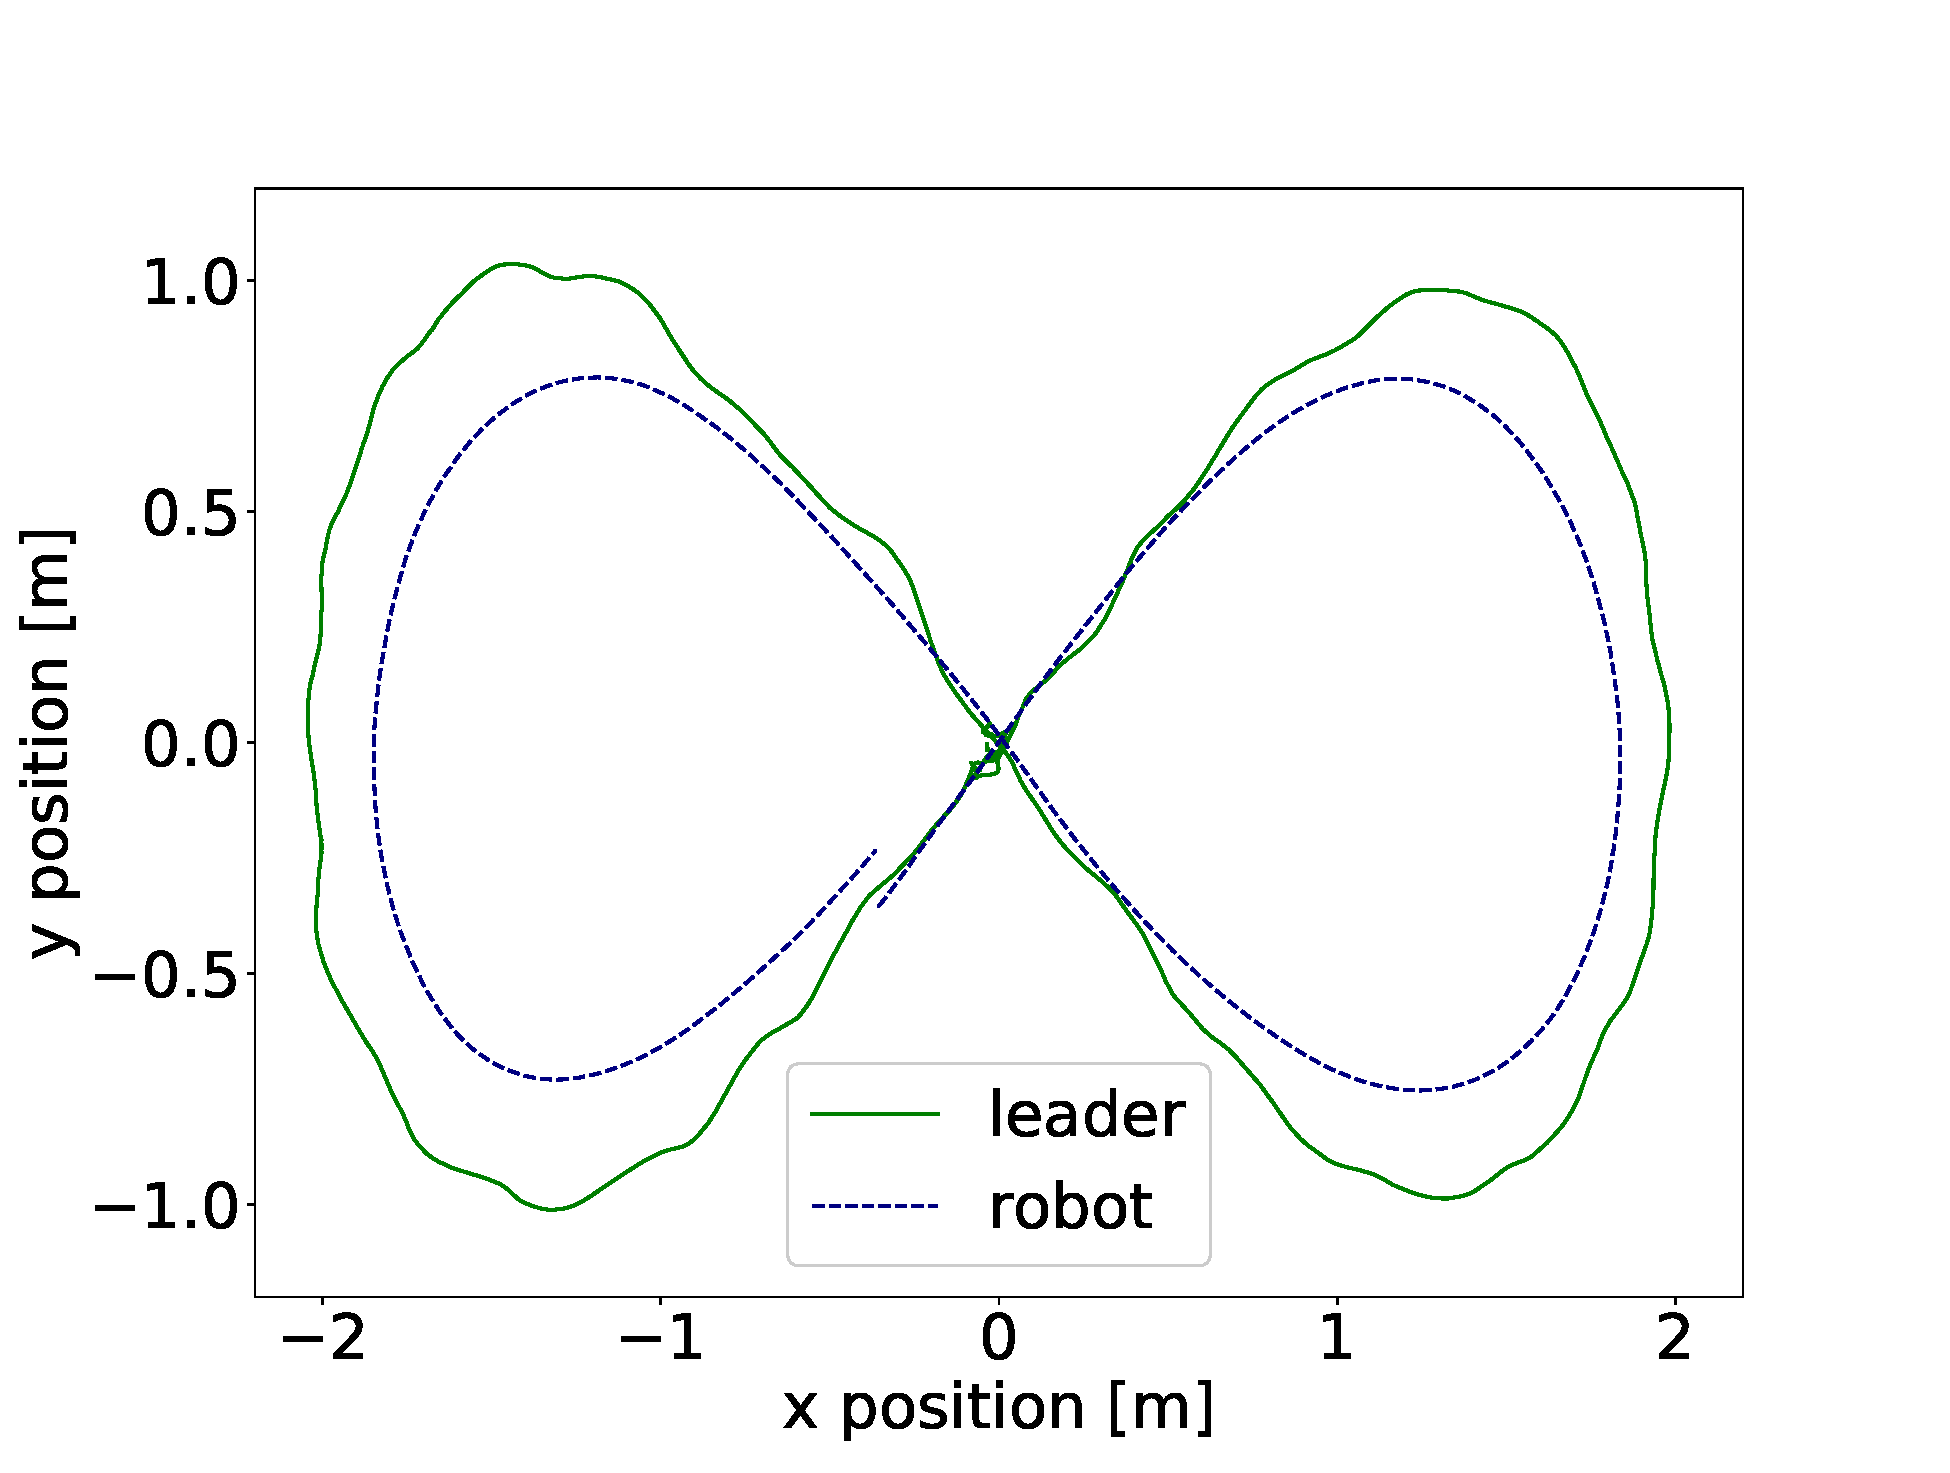
\includegraphics[width=0.8\linewidth]{images/capture_follow-turn.eps}}
    \\
  \caption{Experimentation Results: Trajectories of the leader and follower for \textit{Follow the thread} (a) and \textit{Rotate and go} (b). 
        Speed profiles of the leader and follower for \textit{Follow the thread} (c) and \textit{Rotate and go} (d). 
        (e) Separation distance between robot and leader for both strategies (m).}
  \label{fig:realworldresults} 
\end{figure}


\begin{center}
\begin{tabular}{ |c|c|c|c| }
\hline
$c_v$ & $c_{\alpha}$ & m.t.d. (m) & t.t.d. \\
\hline
\textbf{25}  &   \textbf{20}  & \textbf{0.3876} & \textbf{1.9761}\\
25  &   35  & 0.4672 & 2.3528\\
\hline
\end{tabular}
\captionof{table}{Maximum trajectory deviation m.t.d. and area under normal trajectory deviation t.t.d. in motion capture experiments using \textit{Follow the thread}.}
\label{tab:cap_ft_npd_table}
\end{center}


% \begin{center}
% \begin{tabular}{ |c|c|c|c|c| }
% \hline
% $c_v$ & $c_r$ & $Dt_{off}$ & m.t.d. (m) & t.t.d. \\
% \hline
% 30  &   35  & 0.04  & 0.4116 & 2.8309\\
% \textbf{30}  &   \textbf{35}  & \textbf{0.08 }& \textbf{0.3739} & \textbf{2.0367}\\
% \hline

% \end{tabular}
% \captionof{table}{Maximum trajectory deviation m.t.d. and area under normal trajectory deviation t.t.d. in motion capture experiments using \textit{Rotate and go}.}
% \label{tab:cap_rg_npd_table}
% \end{center}

% We performed an additional simulated experiment to validate whether or not the selected algorithm could be extended to handle weight of the real oxygen tank. A common type of tank used in this type of therapies is a 5 kg oxygen tank.


% We added on the Webots simulation a 5 kg mass on top of our model, and adjusted the coefficients $c_v$ and $c_{\alpha}$ for the  \textit{Follow the thread}  control strategy.  Results are consistent with the outcomes shown previously on Figures~\ref{fig:simulationresults} and~\ref{fig:realworldresults}.  In Figure~\ref{fig:validationwithtank} it can be seen that the shape of the trajectory follows the patient smoothly, the speed profile also follows closely the leader speed, and finally the distance between the patient and the robot is maintained within the safe boundaries.  The obtained metrics are 0.2223 for m.t.d. and 1.1068 for t.t.d. which shows that the following behavior is achieved and verifies, from the simulation perspective, the initial feasibility of the control strategy considering the addition of the oxygen tank.

\section{Discussion}
\label{discussion}

From the leader and robot trajectories in Figure~\ref{fig:simulationresults}(a to d), the control strategy exhibits basic following behavior.  

% For the \textit{Rotate and go} configuration, the parameter $c_r$ affects the dynamic behavior of the robot which needs to be adjusted accordingly.  Lastly, increasing the $Dt_{off}$ from 0.05 to 0.10 made the vehicle less prone to fall behind and produces a better following profile.
%For the \textit{Rotate and go} configuration, a high $c_r$ was important so the robot can turn quickly to point to the leader, but high values of $c_r$ and $c_v$ should be avoided, which may lead to dynamical issues with the inertia affecting the forward direction and missing the leader.  Lastly, increasing the $Dt_{off}$ from 0.05 to 0.10 made the vehicle less prone to fall behind and results in a better following profile.


%From the leader and robot trajectories in Figure \ref{fig:sim_ft_cv15_cr15}, we can see that the robot using \textit{Follow the thread} control exhibits basic following behavior. Deviation occurs when the leader trajectory turns with a tight radius. Comparing different simulations using different values of $c_{\alpha}$, we can also see that the robot tends to miss or cut corners when the leader turns, depending on the value of this constant (figures \ref{fig:sim_ft_cv15_cr5}, \ref{fig:sim_ft_cv15_cr10} and \ref{fig:sim_ft_cv15_cr15}). When $c_{\alpha}$ is low, the robot is slow to turn and makes wider turns, and when it is high, it can turn sharply as soon as the leader starts turning, so it will "cut" the curve. 

%Is was also found that with low $c_v$ values, the robot tends to lag behind the leader when it is going in a straight line, and as a consequence, when the leader turns, the follower is further away and has to make a sharper turn to keep following the leader. Again, a very low values of $c_v$ makes the follower "cut corners", as can be seen in figure \ref{fig:sim_ft_cv5_cr20}.

%The rotateand go We see that this strategy also exhibits a following behavior, although in a more irregular path, as expected, due to the two stage movement algorithm. In this case we evaluated the effects of the constants $c_v$, $c_r$ and $Dt_{off}$. 

%We found that it is important to have a high $c_r$ so the robot turns quickly to point to the leader, or otherwise, as the leader turns, the robot never stops rotating since it takes too much time to get to the point where it can go forward. Therefore, if the leader makes a long turn, the robot never stops rotating and stops following the leader (figure \ref{fig:rgv_cv20_cr5_dr05}).

%However, a very high $c_r$ causes a different issue. When the robot finally points at the leader and starts going forward, if it was rotating too fast, the inertia of the wheels and the robot itself affect the forward movement of the vehicle, which can turn sideways as it tries to go forward in a straight line, diverting the robot from its intended path. A similar thing happens with a very high $c_v$: when the robot stops to rotate, its inertia prevents it from stopping completely and its path is affected as a consequence. This can be seen in figure \ref{fig:rgv_cv35_cr20_dr10}.

%Lastly, we found that calibrating the $Dt_{off}$ parameter also has positive effects in the following performance, since it leaves more margin for the robot to go forward before rotating to point at the leader again. Increasing the $Dt_{off}$ from 0.05 to 0.10 made the vehicle less prone to fall behind and results in a better following (see figure \ref{fig:rg_dt_comp}).



%Both behaviors are described by figures \ref{fig:ft_speed_1} and \ref{fig:rg_speed_1}, which show the speed of the leader and the robot over time.


%When we measured the robot-leader distance over time, we see another significant between the two strategies. As mentioned before, using \textit{Rotate and go}, as the robot rotates, the leader can get further away. Figures \ref{fig:ft_vs_rg_dist} and \ref{fig:ft_vs_rg_dist_hist} show the distance over time and the distribution of distances for each strategy, respectively. 



In line with the simulated results, a similar behavior was found on the experiments performed inside the Motion Capture Lab, and the robot exhibits following behavior for both control strategies as shown on Figure~\ref{fig:realworldresults}.   Although the parameter values obtained from the simulation had to be readjusted for the real world scenario, the relative relation between them was maintained and that helped to narrow the parameter search space.


%We can see that, again, the robot exhibits following behavior. The trajectories in the figures mentioned above show a similar behavior to the one in the software simulation, for both control strategies.

%As in the software simulation, we also evaluated the influence of the algorithm parameters in the robot movement, using the hardware prototype. Figures \ref{fig:ft1_cap_leader_robot} and \ref{fig:ft2_cap_leader_robot} show the robot and leader movement using different values for $c_{\alpha}$. As we have seen in the simulation, a higher $c_{\alpha}$ makes the robot tend to "cut corners" (figure \ref{fig:ft2_cap_leader_robot}).

%For the \textit{Rotate and go} strategy, we compared how different values of $Dt_{off}$ behaved. As we can see in figure \ref{fig:ft2_cap_leader_robot}, a higher $Dt_{off}$ makes the robot less sensitive to leader turns, so the robot has time to move forward and follow the shape of the curve more accurately. 

% As expected, the \textit{Rotate and go} strategy performs a \textit{stop and go} movement, since the vehicle completely stops when rotating to face the leader. This is shown on the speed profiles in Figure~\ref{fig:simulationresults}(c,d) as well as on the real experiment on Figure~\ref{fig:realworldresults}(c,d).   

The smoother movement of the \textit{Follow the thread} algorithm is an additional desired goal, since it can be perceived as less violent or unexpected. %Additionally, when the vehicle stops to rotate, if the leader continues moving, when going forward, the robot might need to accelerate sharply to catch up with the leader, resulting in a sudden movement that can be disturbing for a medical patient or a doctor in the middle of a treatment.

%As it was mentioned before, a smoother movement, with no sudden accelerations, can be desired in the environment where the robot is expected to function, so the \textit{Rotate and go} strategy is better in this respect.

%Another thing to note is that, since the robot has inertia when it tries to stop and rotate (in \textit{Rotate and go}), its speed never gets to  zero as it rotates on its axis. This can also be an issue when following the leader, since the robot can be pushed off its course due to its own movement. 


%As in the simulation, we also see differences in the robot-leader distance over time. The \textit{Rotate and go} strategy performs worse in this respect, reaching higher maximum distances and a higher average distance to the leader (table \ref{tab:cap_ft_vs_rg_dist_table}).

% Finally, regarding the Robot-leader distance r.l.d., the \textit{Rotate and go} strategy results in a less stable distance (higher standard deviation), with higher maximum values, both on the simulated (Figure~\ref{fig:simulationresults}(e)) and on the real world scenario (Figure~\ref{fig:realworldresults}(e)).  This can be specially problematic if we consider the cannula connecting the oxygen tank to the patient, as the cannula has a limited length.  

%These values are also compared in Table \ref{tab:cap_ft_npd_table} and Table~\ref{tab:cap_rg_npd_table}.  

\subsection{Clinical Assessment} 
\label{clinical}

No amount of metrics are enough to evaluate if the robot is a viable solution for this problem or not, without the feedback and the evaluation of the people that are going to physically make use of it. 

ALPI is a non-profit civil association located in Buenos Aires, Argentina, that provides neuromotor rehabilitation for pediatric and adult patients. It was founded in 1943 with the main focus of treating children with poliomyelitis, and has since expanded to deal with all kinds of related diseases. 

Four professional care-givers from ALPI  were invited to test and evaluate the controlling strategy on the prototype.  A live demonstration of the robot working and following a moving person was performed.

In the demonstration, the robot design was outlined and an explanation was given on how the robot worked, how it was built and how to operate it.

Afterwards, health care professionals were invited to use the robot themselves, simulating they were the patient being followed. They used the robot freely to get a general idea of how it behaved, and how it could be used in the rehabilitation process. After all evaluations were finished, various aspects of the vehicle prototype were discussed and then a survey was handed out to document their experience with the robot, and to get their opinion on what other improvements were needed in order to deliver a fully usable product. 

% Survey questions and their averaged numerical evaluations are provided in Table~\ref{tab:alpi_q_table_1}.

% According to their answers, and the discussion we had after testing the robot, the general opinion was that the \textit{Follow the thread} strategy was safer and more convenient for the task. In the survey, when asked \textit{Which of the two strategies is more effective at following the patient in a rehabilitation exercise?}, all 4 people responded that \textit{Follow the thread} is "much better".

% The main concern with the \textit{Rotate and go} strategy was that having to wait for the robot to rotate before moving forward might be unsafe, as the patient could move away from it and compromise the cannula connecting him or her to the oxygen tank. This issue was identified during our own tests, and was not mentioned when explaining the following mechanism to the doctors, to avoid skewing them. They independently identified this problem, and emphasized that it could be a great source of discomfort for the patient.

Another aspect that was remarked from the \textit{Follow the thread} strategy is that since it had a smoother movement, with no sudden stops or accelerations, it was favorable for the stability of the robot in order to carry the heavy oxygen tank.

Two needed security measures were also brought up by the ALPI team. Firstly, the need to add some mechanism for obstacle avoidance. They mentioned the need to have sensors to detect if the robot was about to hit something (specially the patient), and stop immediately, apart from what the control strategy indicated. Secondly, they recognized that some patients have very weak stability, and might fall down or take a step back, towards the robot, so it should be able to automatically move away from the patient, in order not to become another obstacle for her. 

% In order to have more information for the next steps in the development of the robot, we asked for their advise to design the mechanism to attach the threads to the patient being followed. Two ideas were proposed: a belt strapped to the patient waist, or a clasp tied to the clothes of the patient, also near its waistline. The waist is a good attachment point, since it is relatively more stable when the patient moves, compared to its hands or legs, that may make sudden movements and confuse the robot sensors. 


\section{Conclusion and Future Work}
\label{conclusion}

Reescribir esta parte
% From the practical experiments, it is verified that both algorithms ensuing the \textit{following behavior}  in the task of tracking the patient along a lemniscate-shaped trajectory. This following behavior is accomplished with a simple mechanism, a characteristic that significantly keep the price of the device low, putting it within reach of many medical institutions on developing nations.

% Each control strategy has its advantages, but according to various metrics described in this work, the \textit{Follow the thread} strategy had a more desirable behavior, as it tended to follow the leader from a closer distance at all times, while moving in a smooth and predictable way. 

Insightful feedback is gathered from healthcare professionals from ALPI, who provided invaluable data to evaluate the solution. 

% Over all, they highlight the \textit{Follow the thread} strategy as being the safer and more effective one. Most importantly, they also validated the research and were enthusiast about the direction of the project. They proposed a series of improvements and next steps after seeing the prototype in action.

As described in the beginning, it is essential to involve stakeholders such as patients, doctors, nurses, and any other professionals involved in the rehabilitation process early in the design roadmap. They are the ones who understand the problem better than anyone else, and will be the end users of any developed product, as long as it is useful for them.

%The staff at ALPI was enthusiastic about helping in the development of the robot, and their encouragement and support are key reasons to take this project forward.  There are yet many challenges ahead, but these initial results are promising about the viability to develop a real world solution that can improve the quality of life of many people through the use of technology and engineering. 


% \subsection{Validation carrying the oxygen tank}

% In order to advance towards the next step, we performed an additional simulated experiment to validate whether or not the selected algorithm could be extended to  handle the oxygen tank.  ALPI works with 5 kg oxygen tanks, which are manufactured locally.

% We added on the Webots simulation a 5 kg mass on top of our model, and adjusted the coefficients $c_v$ and $c_{\alpha}$ for the  \textit{Follow the thread}  control strategy.  Results are consistent with the outcomes shown previously on Figures~\ref{fig:simulationresults} and~\ref{fig:realworldresults}.  In Figure~\ref{fig:validationwithtank} it can be seen that the shape of the trajectory follows the patient smoothly, the speed profile also follows stringently the leader speed, and finally the distance between the patient and the robot is maintained within the safe boundaries.  The obtained metrics are 0.2223 for m.t.d. and 1.1068 for t.t.d. which shows that the following behavior is achieved and verifies, from the simulation perspective, the initial feasibility of the control strategy considering the addition of the oxygen tank.

\subsection{Future Work}
%A following mechanism has been designed and implemented in a hardware prototype. The mechanism, along with the two control algorithms, has shown promise to be a viable solution to implement in a functioning robot that ALPI, or any other medical institution, can use in their every day exercises with COPD patients. 

The next steps for this project is to scale and iterate the design towards the desired solution, using the data obtained from this experiments and the feedback from care-givers.

\begin{itemize}
    \item Redesign the active spring control mechanism in order to hold the motor temperature in its operational range.
    \item An easy and safe interaction between the patient, the operator and the robot. How to communicate the state of the robot to the operator, how to control and manipulate the robot in an effective and user-friendly way.
    \item Safety measures to keep the patient and the care-giver safe when using the robot. Not only safe from the robot movement, but also from its electronic components.
    \item An obstacle avoidance subsystem. This necessity is emphasized by the personnel from ALPI. The robot should have mechanisms in place to deal with emergency situations, and under no circumstance it can hit the patient or the doctor operating it.
    \item Achieve a battery autonomy that makes the robot useful throughout a complete pulmonary rehabilitation exercise. It is crucial for its usefulness to be able to hold a charge for this period of time, along with the ability to quickly swap batteries if the vehicle will be continually used with different patients.
\end{itemize}{}


% if have a single appendix:
%\appendix[Proof of the Zonklar Equations]
% or
%\appendix  % for no appendix heading
% do not use \section anymore after \appendix, only \section*
% is possibly needed

% use appendices with more than one appendix
% then use \section to start each appendix
% you must declare a \section before using any
% \subsection or using \label (\appendices by itself
% starts a section numbered zero.)
%

% use section* for acknowledgment
% \section{Acknowledgments}
% This project is part of a joint collaboration between ALPI organization and the ITBA University.  Authors would like to thank thoughtfully for the initiative and support given by ALPI, and to the Director of Rehabilitation Technology Dra. Mercedes Molinuevo.  Additionally, authors would also like to offer tremendous gratitude to Natalia Nerina Meda, Soledad Suriá, Eduardo Etcheverry and Sergio Carlos Franco, for the idea of this project and for their invaluable help and enthusiasm to move this project forward.


% \section*{Conflict of Interest Statement}
% The authors declare that the research was conducted in the absence of any commercial or financial relationships that could be construed as a potential conflict of interest.


\bibliographystyle{IEEEtran}
\bibliography{alpibot}

\end{document}
